\begin{frame}[fragile]{The simplified cover tree}

\begin{center}
\begin{tikzpicture}
    [ draw
    , every node/.style={minimum size=10mm,fill=white}
    , level/.style={sibling distance = 23mm/#1, level distance=12mm}
    %,    level distance = 1.5cm}
    , sibling distance=8mm
    ]
\draw (-2.3,0) -- (8.6,0)[dotted];
\draw (-2.3,-12mm) -- (8.6,-12mm)[dotted];
\draw (-2.3,-24mm) -- (8.6,-24mm)[dotted];
\node[shape=circle,draw] at (2.5,0) {10}
    child { node[circle,draw] {8}
        child { node[circle,draw] {7}  }
        child { node[circle,draw] {9} }
        }
    child { node[circle,draw] {12}
        %child { node[circle,draw,fill=lightred,line width=1pt] {9}  }
        %child { node[circle,draw] {13} }
        }
    ;
%\node[shape=circle,draw] at (5,0) {10}
    %child { node[circle,draw] {8}
        %child { node[circle,draw] {7}  }
        %child { node[circle,draw,fill=lightgreen,line width=1pt] {9} }
        %}
    %child { node[circle,draw] {12}
        %child { node[circle,draw,fill=lightgreen,line width=1pt] {11}  }
        %child { node[circle,draw] {13} }
        %}
    %;
\node[fill=none] at (8,3mm) {level 3};
\node[fill=none] at (8,-9mm) {level 2};
\node[fill=none] at (8,-21mm) {level 1};
\end{tikzpicture}
\end{center}

\uncover<1> {
%\vspace{0.15in}
\textbf{The covering invariant.}
For every node $p$, define the function $\covdist p = \exprad p^{\level p}$.
For each child $q$ of $p$
$$
\dist p q \le \covdist p
$$

\vspace{0.15in}
\textbf{The separating invariant.}
For every node $p$, define the function $\sepdist p = \exprad p^{\level p-1}$.
For all distinct children $q_1$ and $q_2$ of $p$
$$
\dist{q_1}{q_2} \ge \sepdist p
$$
}

\uncover<2> {
\vspace{-1.70in}
Advantages of the simplified cover tree:
\vspace{0.05in}
\begin{itemize}
\item Maintains all runtime guarantees of the original cover tree.
\vspace{0.05in}

\item Significantly easier to understand and implement.

%\vspace{0.05in}
The original cover tree was described in terms of an infinitely large tree, only a subset of which actually gets implemented.

\vspace{0.05in}
\item Requires exactly $n$ nodes instead of $O(n)$ nodes.

%\vspace{0.05in}
Fewer nodes means a faster constant factor for all algorithms. %insertions and queries are faster.
\end{itemize}
\vspace{1.3in}
}

\end{frame}


\begin{frame}[fragile]{The simplified cover tree}

\centering
\graphicspath{{slides/covertree/paperimg/}}
% GNUPLOT: LaTeX picture with Postscript
\begingroup
  \makeatletter
  \providecommand\color[2][]{%
    \GenericError{(gnuplot) \space\space\space\@spaces}{%
      Package color not loaded in conjunction with
      terminal option `colourtext'%
    }{See the gnuplot documentation for explanation.%
    }{Either use 'blacktext' in gnuplot or load the package
      color.sty in LaTeX.}%
    \renewcommand\color[2][]{}%
  }%
  \providecommand\includegraphics[2][]{%
    \GenericError{(gnuplot) \space\space\space\@spaces}{%
      Package graphicx or graphics not loaded%
    }{See the gnuplot documentation for explanation.%
    }{The gnuplot epslatex terminal needs graphicx.sty or graphics.sty.}%
    \renewcommand\includegraphics[2][]{}%
  }%
  \providecommand\rotatebox[2]{#2}%
  \@ifundefined{ifGPcolor}{%
    \newif\ifGPcolor
    \GPcolortrue
  }{}%
  \@ifundefined{ifGPblacktext}{%
    \newif\ifGPblacktext
    \GPblacktextfalse
  }{}%
  % define a \g@addto@macro without @ in the name:
  \let\gplgaddtomacro\g@addto@macro
  % define empty templates for all commands taking text:
  \gdef\gplbacktext{}%
  \gdef\gplfronttext{}%
  \makeatother
  \ifGPblacktext
    % no textcolor at all
    \def\colorrgb#1{}%
    \def\colorgray#1{}%
  \else
    % gray or color?
    \ifGPcolor
      \def\colorrgb#1{\color[rgb]{#1}}%
      \def\colorgray#1{\color[gray]{#1}}%
      \expandafter\def\csname LTw\endcsname{\color{white}}%
      \expandafter\def\csname LTb\endcsname{\color{black}}%
      \expandafter\def\csname LTa\endcsname{\color{black}}%
      \expandafter\def\csname LT0\endcsname{\color[rgb]{1,0,0}}%
      \expandafter\def\csname LT1\endcsname{\color[rgb]{0,1,0}}%
      \expandafter\def\csname LT2\endcsname{\color[rgb]{0,0,1}}%
      \expandafter\def\csname LT3\endcsname{\color[rgb]{1,0,1}}%
      \expandafter\def\csname LT4\endcsname{\color[rgb]{0,1,1}}%
      \expandafter\def\csname LT5\endcsname{\color[rgb]{1,1,0}}%
      \expandafter\def\csname LT6\endcsname{\color[rgb]{0,0,0}}%
      \expandafter\def\csname LT7\endcsname{\color[rgb]{1,0.3,0}}%
      \expandafter\def\csname LT8\endcsname{\color[rgb]{0.5,0.5,0.5}}%
    \else
      % gray
      \def\colorrgb#1{\color{black}}%
      \def\colorgray#1{\color[gray]{#1}}%
      \expandafter\def\csname LTw\endcsname{\color{white}}%
      \expandafter\def\csname LTb\endcsname{\color{black}}%
      \expandafter\def\csname LTa\endcsname{\color{black}}%
      \expandafter\def\csname LT0\endcsname{\color{black}}%
      \expandafter\def\csname LT1\endcsname{\color{black}}%
      \expandafter\def\csname LT2\endcsname{\color{black}}%
      \expandafter\def\csname LT3\endcsname{\color{black}}%
      \expandafter\def\csname LT4\endcsname{\color{black}}%
      \expandafter\def\csname LT5\endcsname{\color{black}}%
      \expandafter\def\csname LT6\endcsname{\color{black}}%
      \expandafter\def\csname LT7\endcsname{\color{black}}%
      \expandafter\def\csname LT8\endcsname{\color{black}}%
    \fi
  \fi
  \setlength{\unitlength}{0.0500bp}%
  \begin{picture}(5040.00,3772.00)%
    \gplgaddtomacro\gplbacktext{%
      \csname LTb\endcsname%
      \put(1166,780){\makebox(0,0)[r]{\strut{} 0}}%
      \put(1166,1053){\makebox(0,0)[r]{\strut{} 0.1}}%
      \put(1166,1325){\makebox(0,0)[r]{\strut{} 0.2}}%
      \put(1166,1598){\makebox(0,0)[r]{\strut{} 0.3}}%
      \put(1166,1871){\makebox(0,0)[r]{\strut{} 0.4}}%
      \put(1166,2144){\makebox(0,0)[r]{\strut{} 0.5}}%
      \put(1166,2416){\makebox(0,0)[r]{\strut{} 0.6}}%
      \put(1166,2689){\makebox(0,0)[r]{\strut{} 0.7}}%
      \put(1166,2962){\makebox(0,0)[r]{\strut{} 0.8}}%
      \put(1166,3234){\makebox(0,0)[r]{\strut{} 0.9}}%
      \put(1166,3507){\makebox(0,0)[r]{\strut{} 1}}%
      \put(1661,648){\rotatebox{-45}{\makebox(0,0)[l]{\strut{}yearpredict}}}%
      \put(2023,648){\rotatebox{-45}{\makebox(0,0)[l]{\strut{}twitter}}}%
      \put(2386,648){\rotatebox{-45}{\makebox(0,0)[l]{\strut{}tinyImages}}}%
      \put(2748,648){\rotatebox{-45}{\makebox(0,0)[l]{\strut{}mnist}}}%
      \put(3111,648){\rotatebox{-45}{\makebox(0,0)[l]{\strut{}corel}}}%
      \put(3473,648){\rotatebox{-45}{\makebox(0,0)[l]{\strut{}covtype}}}%
      \put(3836,648){\rotatebox{-45}{\makebox(0,0)[l]{\strut{}artificial40}}}%
      \put(4198,648){\rotatebox{-45}{\makebox(0,0)[l]{\strut{}faces}}}%
      \put(176,2143){\rotatebox{-270}{\makebox(0,0){\strut{}fraction of nodes in the original cover tree }}}%
      \put(396,2143){\rotatebox{-270}{\makebox(0,0){\strut{} required for the simplified cover tree}}}%
    }%
    \gplgaddtomacro\gplfronttext{%
    }%
    \gplbacktext
    \put(0,0){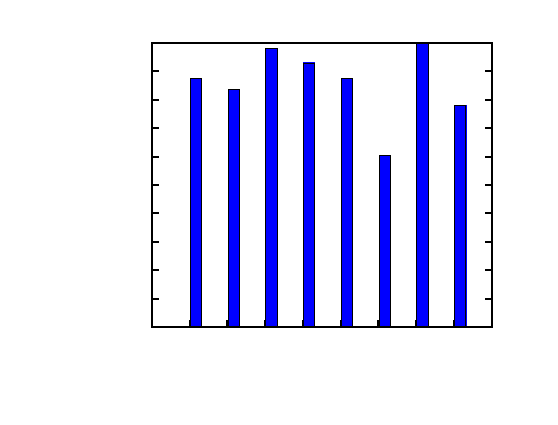
\includegraphics{nodes}}%
    \gplfronttext
  \end{picture}%
\endgroup


\end{frame}
